% ============================================================
% Chapter: Hallucination Reduction with CASAL
% Yang, Qiu, Yu, Zhang, Yang, Kokhlikyan, Cancedda, Garcia-Olano. ICLR 2026.
% ============================================================

% Local color definitions for this chapter
\definecolor{CASALKnownGreen}{RGB}{96,188,173}
\definecolor{CASALUnknownRed}{RGB}{220,107,134}
\newcommand{\known}[1]{\textcolor{CASALKnownGreen}{#1}}
\newcommand{\unknown}[1]{\textcolor{CASALUnknownRed}{#1}}

\blfootnote{This chapter is adapted from: Wannan (Winnie) Yang$^*$, Xinchi Qiu, Lei (Jade) Yu,
Yuchen Zhang, Aobo Yang, Narine Kokhlikyan, Nicola Cancedda, and Diego Garcia-Olano.
``Hallucination Reduction with CASAL: Contrastive Activation Steering for Amortized Learning.''
\textit{International Conference on Learning Representations (ICLR)} (2026).
Wannan Yang is first and corresponding author ($^*$Work done at Meta Superintelligence Labs).
Code: \url{https://github.com/facebookresearch/CASAL}.}

\section*{Abstract}

Large Language Models (LLMs) exhibit impressive capabilities but often hallucinate, confidently providing incorrect answers instead of admitting ignorance. Prior work has shown that models encode linear representations of their own knowledge and that activation steering can reduce hallucinations. These approaches, however, require real-time monitoring and intervention during inference. We introduce \textbf{C}ontrastive \textbf{A}ctivation \textbf{S}teering for \textbf{A}mortized \textbf{L}earning (CASAL), an efficient algorithm that connects interpretability with amortized optimization. CASAL directly bakes the benefits of activation steering into the model's weights during training. Once trained, LLMs answer questions they know while abstaining from answering those they do not. CASAL's lightweight design requires training only a sub-module of a single transformer layer and yet reduces hallucination by $\sim$30\%--40\% across multiple short-form QA benchmarks. CASAL is $\sim$30$\times$ more compute-efficient and $\sim$20$\times$ more data-efficient than strong LoRA-based baselines such as SFT, DPO, and GRPO, boosting its practical applicability in data-scarce domains. Importantly, CASAL also generalizes effectively to out-of-distribution (OOD) domains. We showcase CASAL's flexibility in mitigating hallucinations in both text-only and vision-language models. To our knowledge, CASAL is the first steering-based training method that has been shown to be effective for both dense and Mixture-of-Experts (MoE) architectures. CASAL represents a significant step forward for applying interpretability-inspired methods for scalable and broad deployment in production systems.

\section{Introduction}

Large Language Models (LLMs) have demonstrated near-human or even superhuman intellectual capabilities \citep{brown2020languagemodelsfewshotlearners, ouyang2022traininglanguagemodelsfollow, openai2024gpt4technicalreport}. Yet despite these successes, they sometimes fail in striking ways. A central failure mode is hallucination: the tendency to confidently generate false or unsupported information. Hallucinations undermine trust and restrict the safe deployment of LLMs in real-world settings where factual reliability is critical \citep{rawte2023survey, gekhman2024does, shen2025don}.

Recent interpretability studies---using sparse autoencoder (SAE) features \citep{templeton2024SAEsteering} or residual stream activations \citep{contrastive_activation_addition, turner2024steering}---have revealed that LLMs encode a form of self-knowledge. Specifically, the activations associated with known versus unknown knowledge can be separated along linear directions \citep{calibratinguncertaintylinear, ferrando2025entity}. Moreover, steering these representations reduces overconfidence and enables models to acknowledge uncertainty. However, prior work primarily focuses on inference-time interventions, leaving a significant gap in their practicality as part of scalable alignment pipelines.

\begin{figure}[t]
    \centering
    \includegraphics[width=0.85\linewidth]{figures/ch_casal/fig1_new.png}
    \caption[Overview of the CASAL algorithm]{%
    \textbf{Overview of the CASAL algorithm.}
    (A) \textbf{Knowledge Probing}: CASAL starts by probing the model to figure out what it knows vs. does not know. Multiple responses per query are sampled to classify queries as \known{known} (\known{$\mathcal{D}_{k}$}) or \unknown{unknown} (\unknown{$\mathcal{D}_{u}$}).
    (B) \textbf{Steering}: Difference in means are computed to construct steering vectors (\unknown{$\mathbf{v}^{L^*}_{u}$} and \known{$\mathbf{v}^{L^*}_{k}$}). Target activations ($\unknown{\mathbf{t}^{L^{*}}_{u}}$ and $\known{\mathbf{t}^{L^{*}}_{k}}$) are obtained by adding these steering vectors to the residual stream activation.
    \textbf{Pre-CASAL Behavior}: Prior to training, the model often hallucinates and produces incorrect answers for \unknown{unknown} queries.
    (C) \textbf{CASAL Training}: CASAL training is essentially ``amortized activation steering,'' where instead of repeatedly steering activations online, we train a small subnetwork (a single-layer NN) to approximate the steering solution offline.
    (D) \textbf{Post-CASAL Activations and Behavior}: After training, the model learns a sharper representation with a clearer knowledge boundary. It maintains correct answers on \known{known} queries while abstaining from answering \unknown{unknown} ones.}
    \label{fig:casal}
\end{figure}

If LLMs' internal states already reflect what is known versus unknown, why do they still produce confident but false answers? We hypothesize that a key cause lies in the training and evaluation paradigm of LLMs \citep{knowledgeboundarysurvey, openai2025whyhallucinate}. During pretraining, the language modeling objective rewards predicting the next token given the training corpus distribution, incentivizing plausible continuations even under uncertainty rather than expressions of ignorance. Post-training further amplifies this tendency: the training and evaluation framework optimizes models to be good test-takers, rewarding guessing over acknowledging uncertainty \citep{gekhman2024doesfinetuningllmsnew}.

In this work, we propose an alternative training objective---one that leverages the model's own internal representations to align behavior with knowledge boundaries. Our core hypothesis is that if models are trained to directly utilize their own representations of known and unknown, their generations will better reflect what they truly ``know.'' Concretely, we replace the standard cross-entropy loss with a local representation loss applied to residual stream activations. Whereas cross-entropy loss provides a learning signal from \textit{external} supervision (the training corpus), representation loss provides a learning signal from \textit{within}: the model's own hidden representation.

Importantly, CASAL is among the first approaches to rely solely on a representation-level objective for training LLMs. Prior studies such as RepE \citep{zou2025representationengineering}, ReFAT \citep{yu2024refat}, and others \citep{yu2024mechanistic, ablationfinetuning, chen2025personavectors, representationbending} have explored representation-level fine-tuning, but all employed representation losses as auxiliary signals alongside standard cross-entropy loss. By contrast, \textbf{CASAL treats representation loss as the only and primary optimization objective}, directly teaching the model to utilize its hidden representation.

Our approach connects insights from two fields: interpretability and amortized optimization. Amortized optimization \citep{kingma2013auto, rezende2014stochastic, gershman2014amortized} is a paradigm where costly repeated optimizations are replaced by training a parametric function that approximates the solution. CASAL instantiates this idea by incorporating activation steering into training: it ``amortizes'' the activation steering process by training a lightweight subnetwork that learns to approximate the steering solution, embedding the knowledge boundary directly into the model's weights.

Our main contributions are:
\begin{itemize}
    \item \textbf{Effective Algorithm}: Introducing a training method inspired by interpretability findings and amortized optimization. CASAL enables models to admit ignorance for unknown questions, reducing hallucination rates by $\sim$30\%--40\% across multiple short-form QA benchmarks.
    \item \textbf{Efficiency Gains}: CASAL's objective function enables local and lightweight parameter updates, delivering $\sim$30$\times$ higher compute efficiency (FLOPs per token) and requiring $\sim$20$\times$ less training data (with as little as $\sim$640 training examples) to achieve the same level of performance compared to LoRA-based SFT and DPO.
    \item \textbf{Robust Generalization}: The trained model retains its general capabilities while avoiding excessive refusals. At the same time, it successfully generalizes refusal behavior to unknown queries sampled from out-of-distribution data.
    \item \textbf{Versatility}: CASAL training is modality-agnostic, effectively mitigating hallucination in both text-only and multimodal models.
    \item \textbf{Broad Applicability}: We present the first ever steering-based training framework with general applicability to both dense and Mixture-of-Experts (MoE) models.
\end{itemize}

\section{CASAL}

We now introduce our method, CASAL, which integrates insights from interpretability and amortized optimization to build a lightweight, efficient training framework. The full pipeline is shown in Figure~\ref{fig:casal} and summarized in Algorithm~\ref{alg:casal}. At a high level, CASAL can be understood as an instance of \textit{amortized optimization}: instead of repeatedly solving the steering problem at inference time, we train a parametric subnetwork to approximate this solution once, thereby amortizing the resource use of activation steering across all future queries.

\subsection{Step 1: Knowledge Boundary Probing}

CASAL begins by probing the model to delineate its knowledge boundary. For each input $x \in \mathcal{D}$, we sample $k=10$ completions and compare them to ground-truth answers. For each question, if at least 7 generations are correct, $x$ is labeled as \known{known}; if fewer than 3 are correct, it is labeled as \unknown{unknown}. This produces two subsets: \known{$\mathcal{D}_{k}$} and \unknown{$\mathcal{D}_{u}$}. We adopt a relatively strict threshold $\tau=7$ to ensure high-confidence separation: the model abstains only on knowledge it does not possess, and responds only when it demonstrates consistent correctness. We evaluate CASAL on three datasets: TriviaQA \citep{joshi2017triviaqa}, PopQA \citep{mallen2023popqa}, and EntityQA \citep{ferrando2025entity}.

\subsection{Step 2: Steering}

Next, CASAL constructs contrastive steering vectors to obtain better knowledge boundaries \citep{contrastive_activation_addition, turner2024steering, arditi2024refusal}. For each query $x$, we extract residual stream activations $\mathbf{a}^{L^{*}}(x)$ at a designated target layer $L^{*}$ from the last token position of the question. We then compute mean activations for \known{known} and \unknown{unknown} subsets and construct steering vectors by taking the difference in means, resulting in two vectors: \unknown{$\mathbf{v}^{L^{*}}_{u}$} for abstaining when the model lacks knowledge, and \known{$\mathbf{v}^{L^{*}}_{k}$} for reinforcing correct answering when the model does know. The steering vectors are added to the residual stream activations, yielding target activations \unknown{$\mathbf{t}^{L^{*}}_{u}$} and \known{$\mathbf{t}^{L^{*}}_{k}$}. These target activations are cached and subsequently used to compute the representation loss in Step 3.

\subsection{Step 3: CASAL Training}

Finally, CASAL trains a lightweight \textbf{one-layer network} $M_\text{train}$, initialized with the weight $W^{L^{*}}_{\text{original}}$ from layer $L^{*}$ of the original model. Using a mean squared error objective, CASAL minimizes the distance between current activation $\mathbf{a}^{L^{*}}(x)$ and its corresponding target activation (\known{$\mathbf{t}^{L^{*}}_{k}$} or \unknown{$\mathbf{t}^{L^{*}}_{u}$}). After training, the learned weights $W^{L^*}_{\text{CASAL}}$ are extracted and substituted back into layer $L^*$ of the original model, producing the final model $M_{\text{CASAL}}$. \textbf{Importantly, this representation loss is the sole training objective.} Because this loss is local to layer $L^*$, we only need to train one single layer, in contrast to cross-entropy loss which requires a full forward pass through all layers.

\begin{figure}[htbp]
    \centering
    \begin{algorithm2e}[H]
    \DontPrintSemicolon
    \caption{CASAL: Contrastive Activation Steering for Amortized Learning}
    \label{alg:casal}
    \KwIn{Dataset $\mathcal{D}$; frozen model $M_\text{original}$ with $l$ layers; target layer $L^*$; steering strength $\alpha$; training epochs $E$}
    \BlankLine
    \textbf{STEP 1: Knowledge boundary probing}\;
    Set $k=10$, threshold $\tau=7$\;
    \ForEach{$x \in \mathcal{D}$}{
        Sample $k$ responses $\{y^{(i)}(x)\}$; $s(x)=\sum_i \mathbf{1}[y^{(i)}(x)\text{ correct}]$\;
        \If{$s(x) \ge \tau$}{$\mathcal{D}_{\mathrm{k}} \gets \mathcal{D}_{\mathrm{k}} \cup \{x\}$ \tcp*{\known{``known'' set}}}
        \ElseIf{$k-s(x) \ge \tau$}{$\mathcal{D}_{\mathrm{u}} \gets \mathcal{D}_{\mathrm{u}} \cup \{x\}$ \tcp*{\unknown{``unknown'' set}}}
    }
    \BlankLine
    \textbf{STEP 2: Steering} \tcp*{$\mathbf{a}^{L^*}(x)$: residual activations at layer $L^*$}
    $\mathbf{\bar{a}}^{L^*}_{\mathrm{u}} \gets \frac{1}{|\mathcal{D}_{\mathrm{u}}|}\sum_{x \in \mathcal{D}_{\mathrm{u}}}\mathbf{a}^{L^*}(x)$;\quad $\mathbf{\bar{a}}^{L^*}_{\mathrm{k}} \gets \frac{1}{|\mathcal{D}_{\mathrm{k}}|}\sum_{x \in \mathcal{D}_{\mathrm{k}}}\mathbf{a}^{L^*}(x)$\;
    $\mathbf{v}^{L^*}_{\mathrm{u}} \gets \mathbf{\bar{a}}^{L^*}_{\mathrm{u}}-\mathbf{\bar{a}}^{L^*}_{\mathrm{k}}$;\quad $\mathbf{v}^{L^*}_{\mathrm{k}} \gets \mathbf{\bar{a}}^{L^*}_{\mathrm{k}}-\mathbf{\bar{a}}^{L^*}_{\mathrm{u}}$\;
    $\mathbf{t}^{L^*}_{\mathrm{u}}(x) \gets \mathbf{a}^{L^*}(x) + \alpha \cdot \mathbf{v}^{L^*}_{\mathrm{u}}$, $\forall\, x \in \mathcal{D}_{\mathrm{u}}$ \tcp*{\unknown{``abstain when you don't know''}}
    $\mathbf{t}^{L^*}_{\mathrm{k}}(x) \gets \mathbf{a}^{L^*}(x) + \alpha \cdot \mathbf{v}^{L^*}_{\mathrm{k}}$, $\forall\, x \in \mathcal{D}_{\mathrm{k}}$ \tcp*{\known{``answer when you know''}}
    \BlankLine
    \textbf{STEP 3: CASAL training}\;
    Initialize one-layer network $M_\text{train}$ with weight $W^{L^*}_{\text{original}}$\;
    \For{$e \gets 1$ \KwTo $E$}{
        $\mathcal{L}_{\mathrm{u}} \gets \mathbb{E}_{x\in\mathcal{D}_{\mathrm{u}}}\|\mathbf{t}^{L^*}_{\mathrm{u}}(x)-\mathbf{a}^{L^*}(x)\|^2$\;
        $\mathcal{L}_{\mathrm{k}} \gets \mathbb{E}_{x\in\mathcal{D}_{\mathrm{k}}}\|\mathbf{t}^{L^*}_{\mathrm{k}}(x)-\mathbf{a}^{L^*}(x)\|^2$\;
        Update $M_\text{train}$ weights by $\nabla(\mathcal{L}_{\mathrm{u}}+\mathcal{L}_{\mathrm{k}})$\;
    }
    $M_{\text{CASAL}} \gets M_{\text{original}}$ with $W^{L^*}_{\text{original}}$ replaced by trained $W^{L^*}_{\text{CASAL}}$\;
    \KwOut{Trained model $M_{\text{CASAL}}$}
    \end{algorithm2e}
\end{figure}

\section{CASAL is Effective and Efficient}

We evaluate CASAL against strong baselines including Supervised Fine-Tuning (SFT), Direct Preference Optimization (DPO), and Group Relative Policy Optimization (GRPO), which represent the predominant fine-tuning approaches deployed in production systems today.

\begin{figure}[htbp]
    \centering
    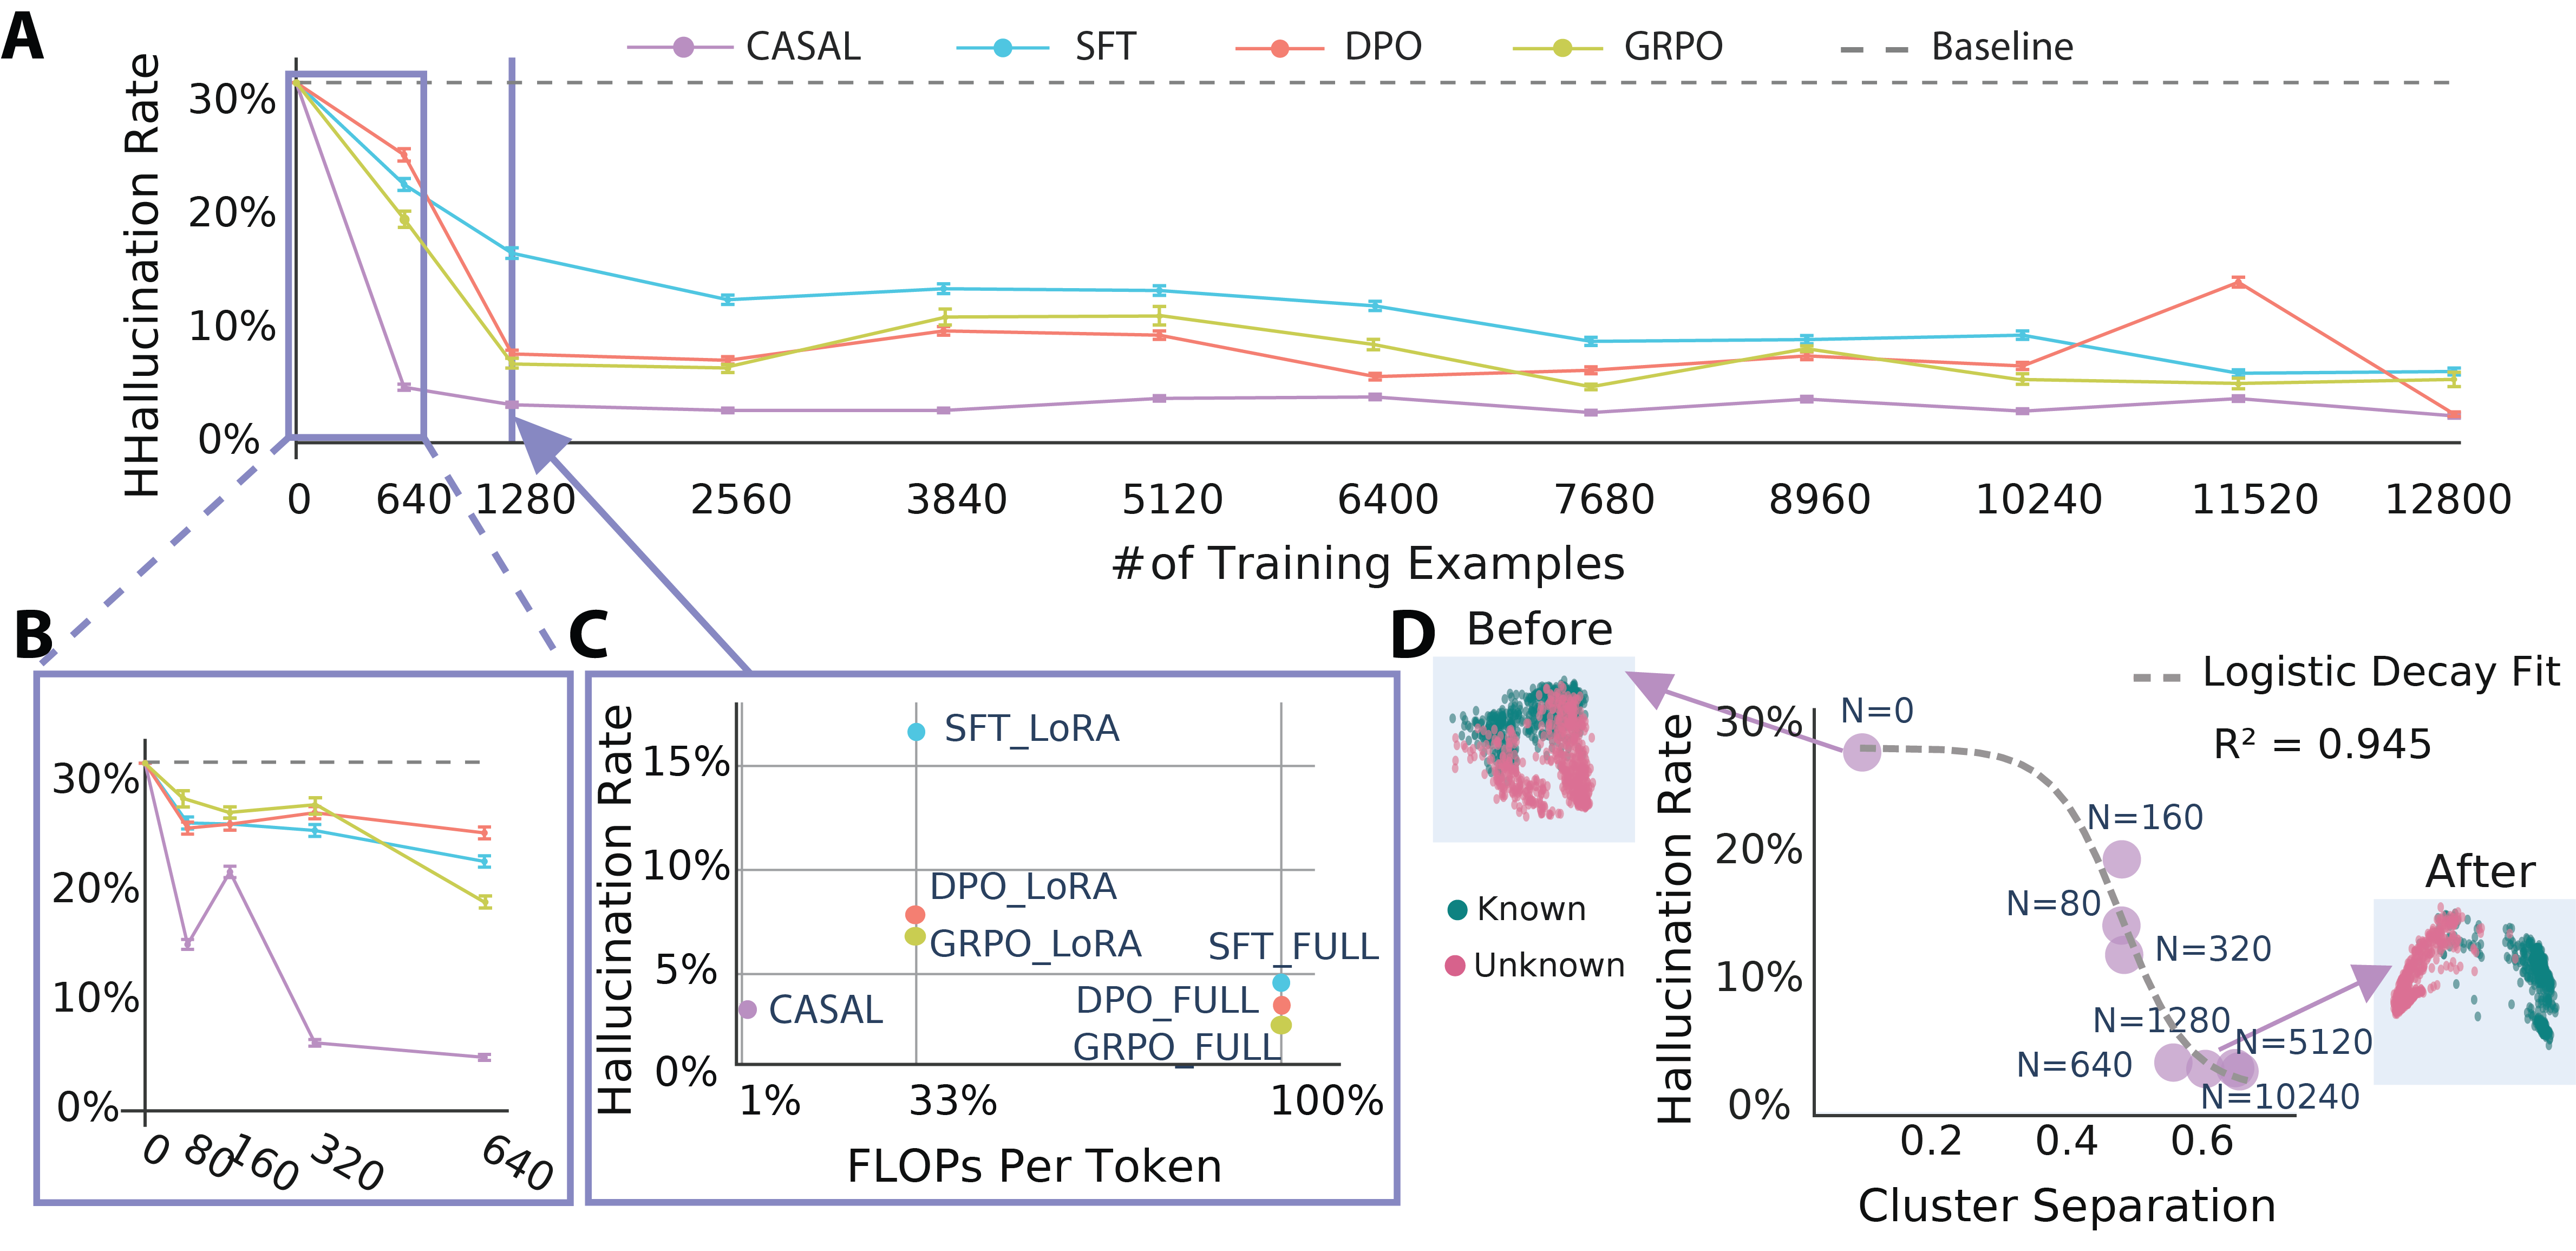
\includegraphics[width=0.85\linewidth]{figures/ch_casal/fig2.png}
    \caption[CASAL is sample-efficient and compute-efficient]{%
    \textbf{CASAL is both sample-efficient and compute-efficient.}
    (A--B) CASAL achieves strong hallucination reduction with orders-of-magnitude fewer training examples comparing to LoRA-based fine-tuning with SFT, DPO and GRPO.
    (C) CASAL is over $30\times$ more compute-efficient than PEFT baselines such as LoRA.
    (D) Hallucination reduction after CASAL training correlates with improved cluster separation between known and unknown queries, measured by silhouette score.}
    \label{fig:efficient}
\end{figure}

\subsection{Sample Efficiency}

We quantify hallucination reduction performance primarily using the \textit{hallucination rate}, which captures the fraction of unknown queries incorrectly attempted by the model. CASAL achieves substantially lower hallucination rates across a wide range of training set sizes. When trained on just 640 examples, CASAL already matches or surpasses the performance of SFT, DPO, and GRPO trained on 12,800 examples (Figure~\ref{fig:efficient}A--B). This translates into more than \textbf{20$\times$ higher data efficiency}, demonstrating that CASAL is especially practical in data-scarce settings.

\subsection{Compute Efficiency}

Beyond sample efficiency, CASAL is also highly compute efficient. By updating only a lightweight sub-module within a single transformer layer, CASAL is substantially more compute efficient than full fine-tuning or even LoRA-based parameter-efficient fine-tuning (PEFT). As shown in Figure~\ref{fig:efficient}C, CASAL achieves lower hallucination rates while requiring over \textbf{30$\times$ fewer FLOPs per token} than LoRA during training. This efficiency stems from two key properties: because CASAL's loss is local to layer $L^*$, forward and backward passes operate exclusively within the single-layer network $M_\text{train}$; and CASAL computes loss at a single position (the last token of the question), whereas SFT and DPO average loss over all generated tokens.

\subsection{Learning Better Knowledge Boundaries}

By training with a local representation loss, CASAL encourages clearer separation between activations corresponding to known and unknown queries. As shown in Figure~\ref{fig:efficient}D, silhouette scores increase as training progresses, and this separation is correlated with the reduction in hallucination rate. The strong correspondence (logistic fit, $R^2 = 0.945$) between representational separation and behavioral outcomes indicates that CASAL's effectiveness arises from more faithfully encoding and utilizing knowledge boundaries.

\section{CASAL Preserves Model Capability}

An important requirement for any practically useful hallucination-reduction method is that it should not degrade a model's general capabilities nor induce excessive refusals on queries the model can correctly answer.

\begin{table}[htbp]
\centering
\small
\resizebox{\textwidth}{!}{%
\begin{tabular}{l c c c c c c}
\toprule
\textbf{Methods} &
\multicolumn{3}{c}{\textbf{Refusal Rate ($\downarrow$)}} &
\multicolumn{3}{c}{\textbf{Accuracy ($\uparrow$)}} \\
\cmidrule(lr){2-4} \cmidrule(lr){5-7}
& \textbf{PopQA} & \textbf{TriviaQA} & \textbf{EntityQA}
& \textbf{PopQA} & \textbf{TriviaQA} & \textbf{EntityQA} \\
\midrule
Baseline & \textbf{18.19\%$\pm$3.01} & 7.93\%$\pm$1.14 & 8.94\%$\pm$2.18
         & \textbf{91.08\%$\pm$2.23} & \textbf{95.82\%$\pm$2.24} & 88.59\%$\pm$1.46 \\
\midrule\midrule
SFT      & 20.32\%$\pm$1.09 & 10.01\%$\pm$1.16 & 11.08\%$\pm$1.24
         & 82.89\%$\pm$1.33 & 92.45\%$\pm$1.29 & 85.75\%$\pm$1.18 \\
DPO      & 21.79\%$\pm$1.11 & 14.37\%$\pm$2.06 & 17.66\%$\pm$2.14
         & 90.25\%$\pm$1.06 & 95.30\%$\pm$0.96 & 89.84\%$\pm$1.16 \\
GRPO     & 17.48\%$\pm$4.46 & 17.77\%$\pm$3.82 & 16.67\%$\pm$4.42
         & 85.78\%$\pm$4.36 & 91.67\%$\pm$2.76 & 85.48\%$\pm$3.52 \\
CASAL    & 19.89\%$\pm$1.15 & \textbf{7.29\%$\pm$1.34} & \textbf{6.84\%$\pm$1.23}
         & 85.11\%$\pm$1.88 & 95.34\%$\pm$2.25 & \textbf{89.90\%$\pm$0.99} \\
\bottomrule
\end{tabular}}
\caption[CASAL does not introduce over-refusal on known queries]{CASAL does not introduce over-refusal nor degrade performance for \known{known} queries. Refusal rate and accuracy across three different QA datasets are measured.}
\label{tab:over_refusal}
\end{table}

Table~\ref{tab:over_refusal} reports refusal rates on three QA datasets. CASAL achieves the lowest refusal rates on TriviaQA (7.29\%) and EntityQA (6.84\%), while maintaining a competitive rate on PopQA (19.89\%). These results demonstrate that CASAL reduces hallucination on unknown queries without over-penalizing the model into unnecessary refusals for known ones.

\begin{table}[htbp]
\centering
\small
\begin{tabularx}{\linewidth}{l *{3}{X} X}
\toprule
\textbf{Methods} &
\multicolumn{3}{c}{\textbf{Accuracy ($\uparrow$)}} &
\multicolumn{1}{c}{\textbf{Win rate ($\uparrow$)}} \\
\cmidrule(lr){2-4}\cmidrule(lr){5-5}
& \textbf{MMLU} & \textbf{GSM8K} & \textbf{GPQA} & \textbf{MT Bench} \\
& \textbf{(General)} & \textbf{(Math)} & \textbf{(Reasoning)} & \textbf{(Coherence)} \\
\midrule
Baseline & 68.01$\pm$0.34 & 77.48$\pm$1.15 & \textbf{33.31$\pm$0.34} & 7.38$\pm$0.06 \\
\midrule\midrule
SFT      & 67.90$\pm$0.23 & 75.66$\pm$1.18 & 32.82$\pm$0.34 & 7.44$\pm$0.13 \\
DPO      & 68.03$\pm$0.26 & \textbf{78.16$\pm$1.14} & 31.43$\pm$0.37 & 7.39$\pm$0.15 \\
GRPO     & 67.73$\pm$0.38 & 76.66$\pm$1.21 & 31.92$\pm$0.22 & 7.44$\pm$0.11 \\
CASAL    & \textbf{68.04$\pm$0.44} & 77.02$\pm$1.16 & 33.18$\pm$0.34 & \textbf{7.57$\pm$0.08} \\
\bottomrule
\end{tabularx}
\caption[CASAL preserves general capability]{CASAL preserves general capability. Performances on general knowledge (MMLU), math (GSM8K), reasoning (GPQA), and context-aware multi-turn conversational ability (MT-Bench) are measured. Higher is better.}
\label{tab:general_capability}
\end{table}

We further assess models' general capability including MMLU \citep{mmlu} for general knowledge, GSM8K \citep{gsm8k} for math reasoning, GPQA \citep{gpqa} for scientific reasoning, and MT-Bench \citep{mtbench} for coherence in multi-turn conversations. As shown in Table~\ref{tab:general_capability}, CASAL performs on par with strong baselines across all metrics, demonstrating that it reduces hallucinations on unknown queries while avoiding over-refusal on known queries without sacrificing general capability.

\section{CASAL is OOD Generalizable}

Does CASAL capture a generalizable notion of what the model knows versus does not know beyond its training distribution? We test its ability to generalize across both in-distribution and out-of-distribution (OOD) settings.

\begin{table}[htbp]
\centering
\small
\resizebox{\textwidth}{!}{%
\begin{tabular}{l l c c c c c c}
\toprule
\textbf{Dataset} & \textbf{Methods} &
\multicolumn{2}{c}{\textbf{\unknown{Hallucination Rate (Unknown)} ($\downarrow$)}} &
\multicolumn{2}{c}{\textbf{\known{Refusal Rate (Known)} ($\downarrow$)}} &
\multicolumn{2}{c}{\textbf{\known{Accuracy (Known)} ($\uparrow$)}} \\
\cmidrule(lr){3-4}\cmidrule(lr){5-6}\cmidrule(lr){7-8}
& & \textbf{Train} & \textbf{Test}
& \textbf{Train} & \textbf{Test}
& \textbf{Train} & \textbf{Test} \\
\midrule
TriviaQA & Baseline & 48.20\%$\pm$1.34 & 50.74\%$\pm$1.12 & 9.06\%$\pm$0.93 & \textbf{7.93\%$\pm$2.02} & \textbf{94.22\%$\pm$1.44} & \textbf{95.82\%$\pm$1.22} \\
(Wiki vs. Web) & SFT  & 24.44\%$\pm$1.65 & 35.44\%$\pm$1.64 & 14.77\%$\pm$1.52 & 15.10\%$\pm$1.77 & 91.23\%$\pm$0.54 & 90.26\%$\pm$1.15 \\
& DPO  & 23.28\%$\pm$1.02 & 33.77\%$\pm$0.99 & 13.62\%$\pm$1.08 & 16.33\%$\pm$1.19 & 90.23\%$\pm$1.09 & 88.13\%$\pm$1.30 \\
& GRPO  & 22.33\%$\pm$1.34 & 33.12\%$\pm$1.88 & 15.99\%$\pm$1.30 & 18.10\%$\pm$1.09 & 88.83\%$\pm$0.96 & 87.27\%$\pm$1.03 \\
& CASAL  & \textbf{20.47\%$\pm$1.11} & \textbf{32.42\%$\pm$1.29} & \textbf{8.28\%$\pm$1.16} & 11.69\%$\pm$2.22 & 92.03\%$\pm$0.82 & 90.08\%$\pm$1.33 \\
\midrule
PopQA & Baseline & 74.87\%$\pm$2.92 & 74.35\%$\pm$1.56 & 18.95\%$\pm$1.39 & \textbf{18.19\%$\pm$1.46} & \textbf{90.84\%$\pm$1.51} & \textbf{91.08\%$\pm$0.92} \\
(Group 1 vs. 2) & SFT  & 22.77\%$\pm$1.08 & 24.02\%$\pm$1.11 & 14.04\%$\pm$1.16 & 20.88\%$\pm$1.09 & 85.01\%$\pm$1.06 & 85.74\%$\pm$1.60 \\
& DPO  & 21.08\%$\pm$1.33 & 24.88\%$\pm$0.99 & 14.99\%$\pm$1.62 & 19.19\%$\pm$1.55 & 84.66\%$\pm$0.90 & 84.01\%$\pm$1.11 \\
& GRPO  & 20.19\%$\pm$1.05 & 24.22\%$\pm$1.32 & 18.07\%$\pm$1.02 & 21.10\%$\pm$1.33 & 80.13\%$\pm$0.31 & 80.98\%$\pm$1.06 \\
& CASAL  & \textbf{22.48\%$\pm$1.45} & \textbf{23.42\%$\pm$1.94} & \textbf{13.97\%$\pm$1.78} & 19.10\%$\pm$1.30 & 85.23\%$\pm$0.86 & 84.27\%$\pm$1.99 \\
\bottomrule
\end{tabular}}
\caption[CASAL generalizes across data sources and groups]{CASAL learns a generalizable notion of \known{known} vs.\ \unknown{unknown}, transferring between data sources within TriviaQA (Wikipedia vs.\ Web) and across groups within PopQA.}
\label{tab:generalization_within}
\end{table}

As shown in Table~\ref{tab:generalization_within}, CASAL trained on Wikipedia-style data generalizes effectively to web data, reducing hallucination rate from 50.7\% to 32.4\% while maintaining high accuracy on known queries (92.0\% vs.\ 95.8\%). A similar trend is observed on PopQA, where CASAL substantially reduces hallucinations in both groups. These results indicate that CASAL does not simply memorize steering directions but learns a transferable notion of known versus unknown knowledge.

\begin{table}[htbp]
\centering
\small
\resizebox{\textwidth}{!}{%
\begin{tabular}{l c c c c c c}
\toprule
\textbf{Methods} &
\multicolumn{2}{c}{\textbf{\unknown{Hallucination Rate} ($\downarrow$)}} &
\multicolumn{2}{c}{\textbf{\known{Refusal Rate} ($\downarrow$)}} &
\multicolumn{2}{c}{\textbf{\known{Accuracy} ($\uparrow$)}} \\
\cmidrule(lr){2-3}\cmidrule(lr){4-5}\cmidrule(lr){6-7}
& \textbf{TriviaQA (Train)} & \textbf{EntityQA (Test)}
& \textbf{TriviaQA (Train)} & \textbf{EntityQA (Test)}
& \textbf{TriviaQA (Train)} & \textbf{EntityQA (Test)} \\
\midrule
Baseline & 48.2\%$\pm$1.33 & 50.74\%$\pm$0.92 & \textbf{9.06\%$\pm$1.22} & \textbf{12.89\%$\pm$1.49} & \textbf{94.22\%$\pm$0.93} & \textbf{95.82\%$\pm$2.32} \\
\midrule\midrule
SFT  & 30.63\%$\pm$1.53 & 23.13\%$\pm$1.66 & 21.16\%$\pm$1.34 & 29.84\%$\pm$1.40 & 88.80\%$\pm$1.33 & 80.77\%$\pm$1.05 \\
DPO  & 20.63\%$\pm$2.21 & 18.30\%$\pm$1.45 & 13.89\%$\pm$1.22 & 22.02\%$\pm$1.29 & 92.91\%$\pm$1.06 & 87.41\%$\pm$1.22 \\
GRPO & \textbf{14.00\%$\pm$0.55} & 12.83\%$\pm$4.18 & 21.43\%$\pm$4.10 & 17.25\%$\pm$5.56 & 85.69\%$\pm$8.75 & 85.24\%$\pm$4.32 \\
CASAL & 18.23\%$\pm$1.03 & \textbf{11.72\%$\pm$1.66} & 9.29\%$\pm$1.48 & 13.82\%$\pm$1.55 & 93.36\%$\pm$1.47 & 95.77\%$\pm$1.64 \\
\bottomrule
\end{tabular}}
\caption[CASAL generalizes across datasets (TriviaQA to EntityQA)]{CASAL supports OOD generalization across datasets. The model is trained on TriviaQA and tested on EntityQA as an out-of-distribution setting. Hallucination rate drops from 50.7\% to 11.7\% on the unseen dataset.}
\label{tab:generalization_across}
\end{table}

We next evaluate a stronger OOD setting: training CASAL on TriviaQA and evaluating on a completely different dataset (EntityQA). As shown in Table~\ref{tab:generalization_across}, hallucination rate on the unseen EntityQA dataset drops from 50.7\% to 11.7\%, while accuracy on known queries remains above 95\%. This demonstrates that CASAL's learned representations capture knowledge boundaries that remain robust even under OOD transfer.

\section{CASAL is Modality- and Architecture-Agnostic}

\subsection{CASAL Reduces Hallucination in Vision-Language Models}

We apply CASAL to a vision-language model (Qwen2.5-VL-7B-Instruct \citep{qwen2024qwen2}) and train on the WorldCuisines-VQA \citep{winata2024worldcuisines} and Landmark-VQA datasets. CASAL reduces hallucination rate by 38.74\% on WorldCuisines-VQA and 44.53\% on Landmark-VQA, while accuracy on known queries is preserved (Table~\ref{tab:vision}). This confirms that CASAL's mechanism for sharpening knowledge boundaries extends naturally to multimodal models.

\begin{table}[htbp]
\centering
\small
\begin{tabular}{l c cc}
\toprule
\textbf{Methods} &
\multicolumn{3}{c}{\textbf{WorldCuisines-VQA}} \\
\cmidrule(lr){2-4}
& \textbf{\unknown{Hallucination Rate ($\downarrow$)}} &
\textbf{\known{Refusal Rate ($\downarrow$)}} &
\textbf{\known{Accuracy ($\uparrow$)}} \\
\midrule
Baseline & 72.35\%$\pm$1.77 & \textbf{13.91\%$\pm$1.37} & 76.72\%$\pm$1.67 \\
\midrule\midrule
SFT  & 35.05\%$\pm$2.87 & 24.33\%$\pm$2.76 & 87.42\%$\pm$1.66 \\
DPO  & 36.44\%$\pm$3.77 & 24.02\%$\pm$2.11 & 86.66\%$\pm$1.74 \\
GRPO  & 35.19\%$\pm$2.99 & 28.73\%$\pm$2.73 & 80.18\%$\pm$1.64 \\
CASAL  & \textbf{33.34\%$\pm$3.13} & 25.44\%$\pm$2.91 & \textbf{90.36\%$\pm$1.96} \\
\bottomrule
\end{tabular}
\quad
\begin{tabular}{l c cc}
\toprule
\textbf{Methods} &
\multicolumn{3}{c}{\textbf{Landmark-VQA}} \\
\cmidrule(lr){2-4}
& \textbf{\unknown{Hallucination Rate ($\downarrow$)}} &
\textbf{\known{Refusal Rate ($\downarrow$)}} &
\textbf{\known{Accuracy ($\uparrow$)}} \\
\midrule
Baseline & 75.78\%$\pm$1.69 & 3.59\%$\pm$0.73 & 90.80\%$\pm$1.55 \\
\midrule\midrule
SFT  & 39.05\%$\pm$4.07 & 2.64\%$\pm$3.01 & 92.77\%$\pm$1.42 \\
DPO  & 35.99\%$\pm$1.03 & 6.06\%$\pm$1.44 & 94.11\%$\pm$1.01 \\
GRPO  & 35.44\%$\pm$1.81 & 8.19\%$\pm$1.09 & 90.75\%$\pm$1.31 \\
CASAL  & \textbf{31.25\%$\pm$8.32} & \textbf{3.12\%$\pm$3.01} & \textbf{99\%$\pm$0.03} \\
\bottomrule
\end{tabular}
\caption[CASAL reduces hallucination in vision-language models]{CASAL is modality-agnostic. It reduces hallucination in a vision-language model (Qwen2.5-VL-7B-Instruct) on WorldCuisines-VQA (left) and Landmark-VQA (right).}
\label{tab:vision}
\end{table}

\subsection{CASAL Reduces Hallucination in Mixture-of-Experts Models}

MoE models pose a unique challenge since knowledge and uncertainty may be distributed across different experts. We investigated how unknown versus known queries are represented across experts in the OLMoE model \citep{muennighoff2025olmoeopenmixtureofexpertslanguage}. As illustrated in Figure~\ref{fig:moe}, activations for known and unknown queries are mostly co-represented in the same experts. CASAL applies a local representation loss on the residual stream activations with converging signal across all experts. After training, residual stream activations show a much clearer boundary between known and unknown queries. Hallucination rate for unknown queries drops by 42.9\%, while accuracy on known queries remains unchanged (Figure~\ref{fig:moe}D).

\begin{figure}[htbp]
    \centering
    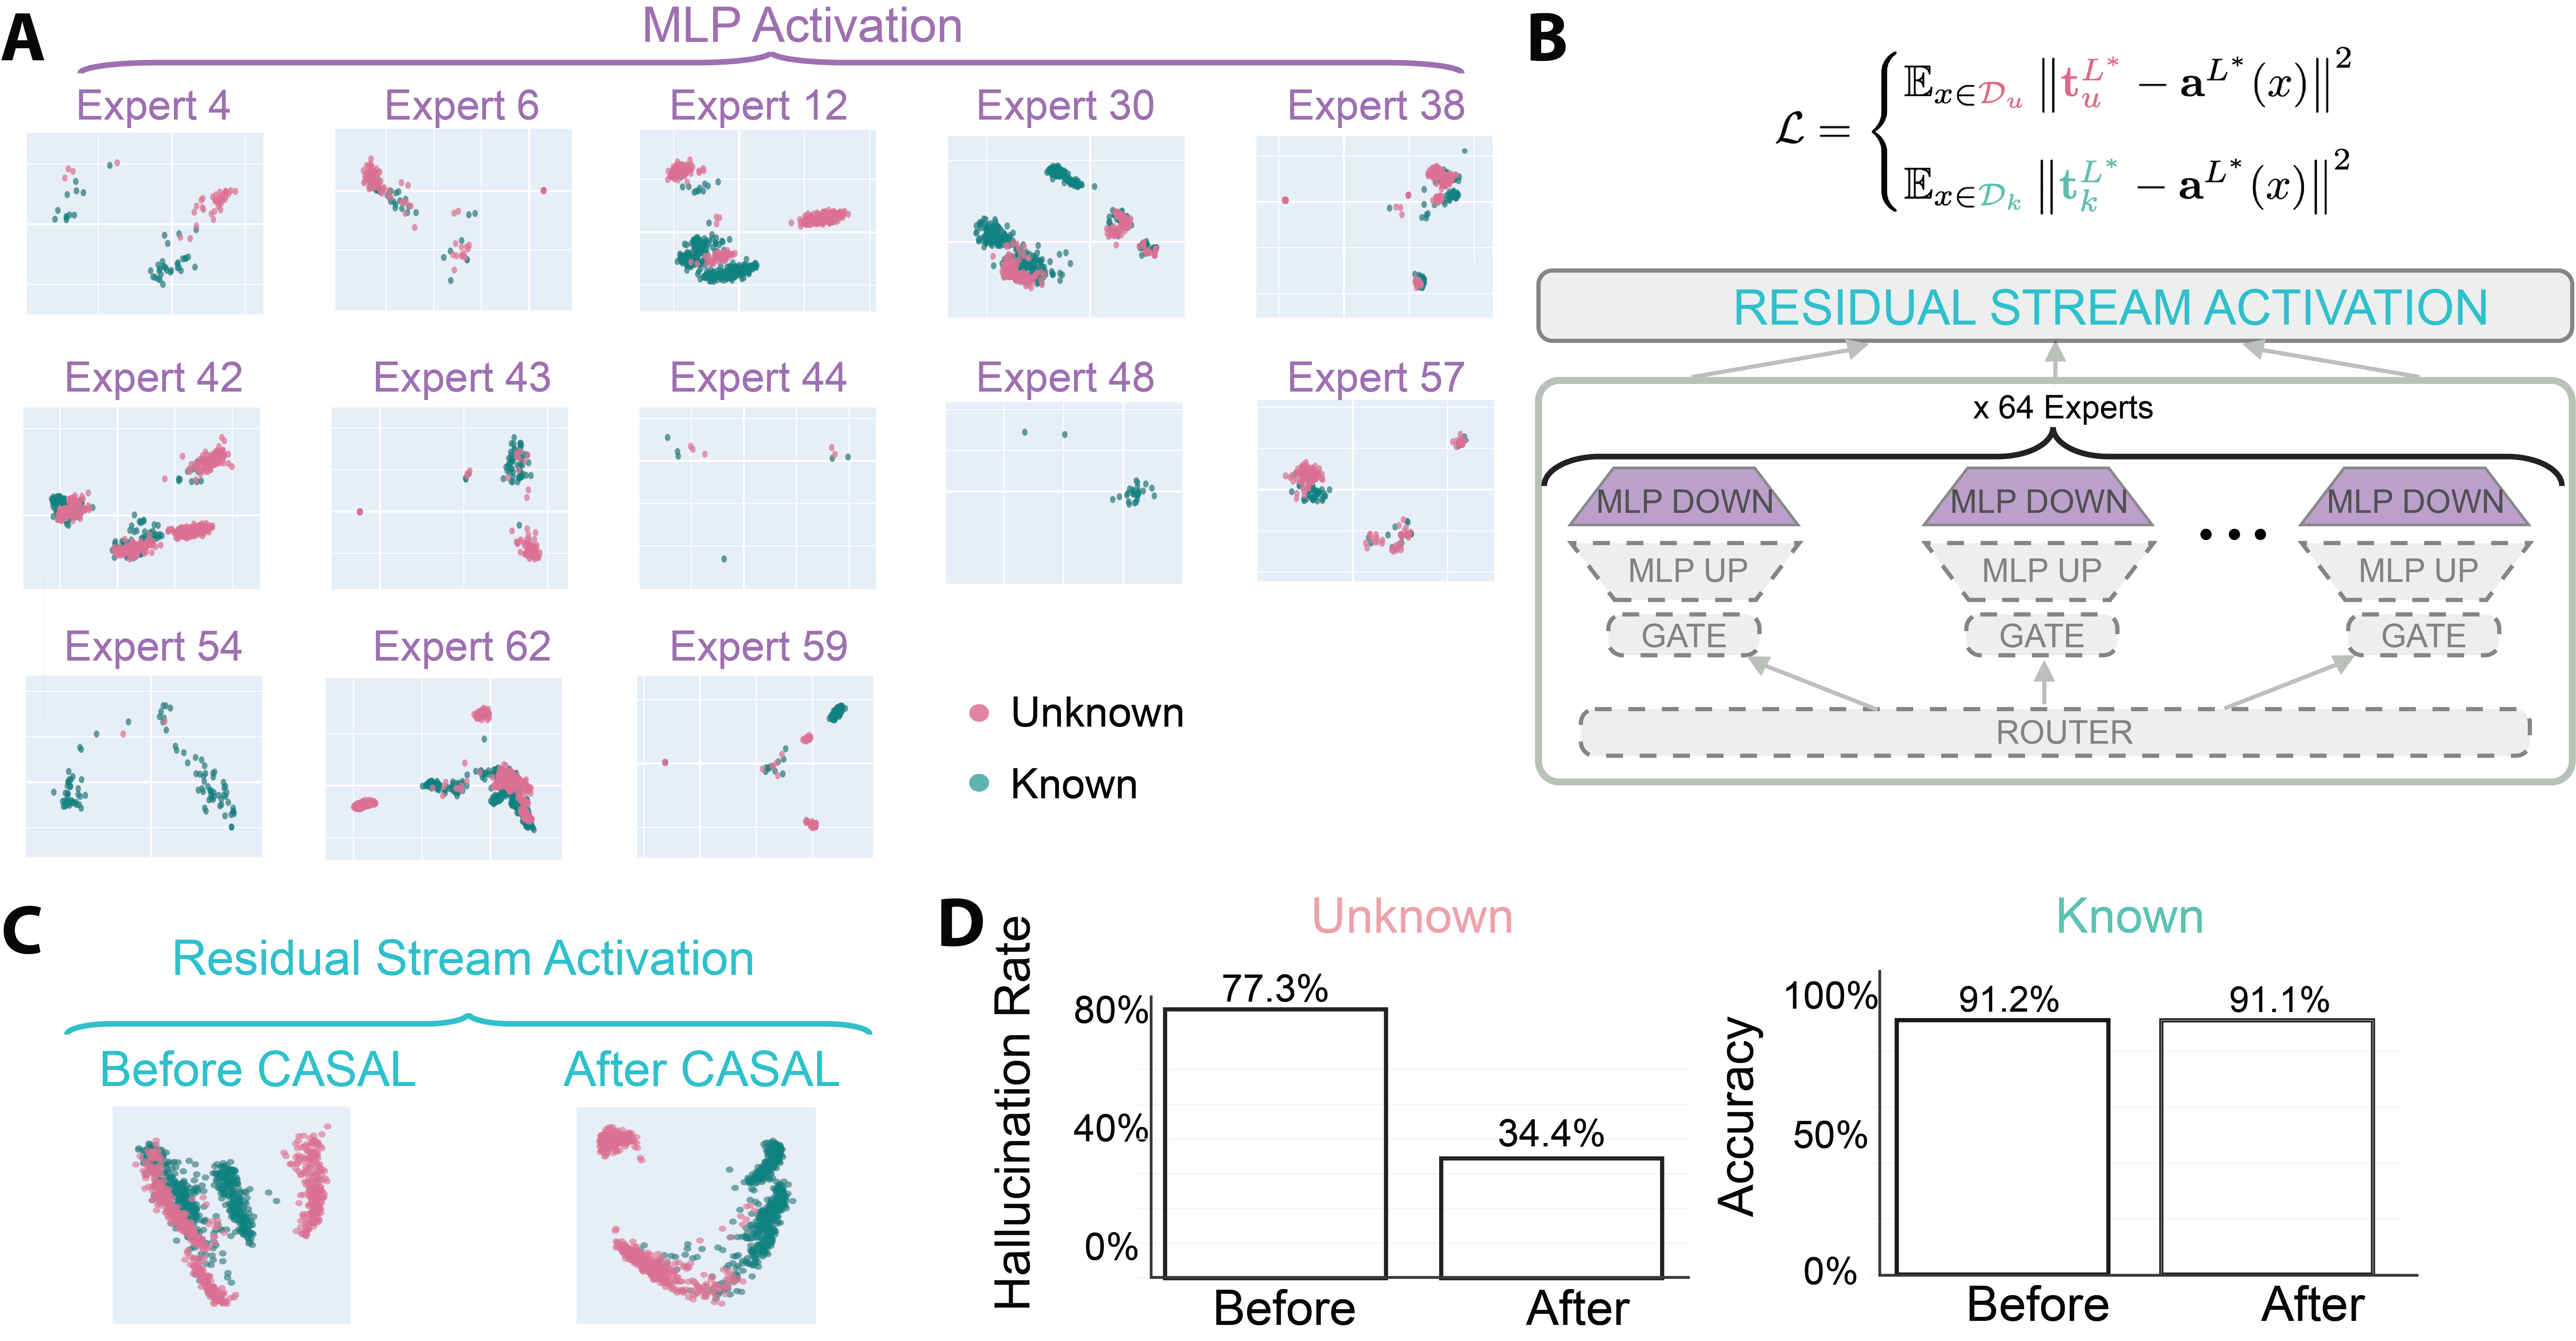
\includegraphics[width=0.92\linewidth]{figures/ch_casal/moe/moe.png}
    \caption[CASAL reduces hallucination in Mixture-of-Experts models]{%
    \textbf{CASAL is architecture-agnostic.} It effectively reduces hallucination for OLMoE.
    (A) Visualization of MLP activations from different experts in a MoE model before CASAL training.
    (B) CASAL applies a local representation loss on residual stream activations. During training, weights are updated on only a lightweight sub-module across experts.
    (C) Residual stream activations before and after CASAL training.
    (D) CASAL reduces hallucination rate on unknown queries while maintaining low refusal score and high accuracy for known queries.}
    \label{fig:moe}
\end{figure}

These results establish that CASAL is both \textit{architecture-agnostic} and \textit{modality-agnostic}. Whether applied to dense or MoE transformers, or to text-only versus vision-language models, CASAL consistently reduces hallucination rates while maintaining high accuracy.

\section{Related Work}

\paragraph{Hallucination Mitigation.} Steering-based approaches \citep{contrastive_activation_addition, turner2024steering} for hallucination reduction typically apply interventions during inference \citep{ferrando2025entity, calibratinguncertaintylinear, li2024inferencetimeinterventionelicitingtruthful, latentshallucination}, introducing extra computational overhead during deployment. In contrast, CASAL eliminates the need for per-instance intervention by directly baking the knowledge boundaries into model parameters. A complementary body of work modifies model parameters to encourage calibrated abstention and reduce hallucination \citep{KnowledgeBoundary, linguisticcalibration, chen2025personavectors}. Compared to these efforts, CASAL provides the first general steering-based training framework broadly applicable to both dense and sparse (MoE) architectures.

\paragraph{Amortized Optimization.} Amortized optimization \citep{kingma2013auto, rezende2014stochastic, gershman2014amortized} replaces expensive repeated optimization with a parametric function trained to approximate the solution. CASAL can be viewed as \textit{amortized activation steering}, where the resource-intensive process of online steering is distilled into a lightweight subnetwork trained offline and reused at inference \citep{amos2025tutorialamortizedoptimization}.

\paragraph{Activation Steering and Representation Learning.} A line of work has focused on inference-time interventions, applying steering vectors dynamically to control model behavior \citep{calibratinguncertaintylinear, li2024inferencetimeinterventionelicitingtruthful, arditi2024refusal}. A parallel line shapes internal representations during finetuning \citep{tian2025representationengineeringvisual, yu2024mechanistic, chen2025personavectors, ablationfinetuning}, including representation fine-tuning (ReFT) \citep{wu2024reftrepresentationfinetuning} and representation engineering (RepE) \citep{zou2025representationengineering}. CASAL differs from all of these by using representation loss as the \textit{sole} training objective.

\section{Conclusion and Limitations}

We introduced CASAL, a lightweight, effective, and broadly applicable method for reducing hallucinations in large language models. By embedding knowledge boundaries directly into model weights, CASAL achieves substantial reductions in hallucination without degrading general capabilities, while being markedly more compute- and data-efficient than standard baselines. Beyond its empirical results, CASAL provides initial evidence of a broader principle: insights from interpretability can be distilled into training objectives that scale.

Several limitations remain. First, although CASAL generalizes across short-form QA datasets, modalities, and architectures, its effectiveness in reasoning models remains to be systematically tested. Second, our evaluation focuses on hallucinations in short-form QA tasks; exploring effectiveness in long-form generation represents an important future direction. Third, one particularly exciting future direction is the integration of CASAL into LLM-based agentic systems. As LLMs become tool-using agents integrated into everyday workflows, their reliability becomes critical---misplaced confidence can lead to cascading errors. CASAL's mechanism for sharpening knowledge boundaries could therefore serve as a component for more reliable agentic systems, enabling agents to make better decisions about when to respond directly versus when to invoke external tools.

\subsection*{Acknowledgments}

We thank Nathaniel Li, Irene Zhang, Julian Coda-Forno, Sriyash Poddar, Anselm Paulus, Sai Surya Duvvuri, Rachit Bansal, Devvrit Khatri, Ellie Pavlick, and Jojo Yang for providing thoughtful feedback and insightful discussions on the manuscript.
